\documentclass[a4paper, 10pt]{report}
%\usepackage{showframe}
\usepackage{amsmath, amssymb, amsthm}
\usepackage[english]{babel}
\usepackage[utf8]{inputenc} %this package is used by \tableofcontents   
\usepackage{comment} %\begin{comment}...\end{comment} 
\usepackage{mathrsfs} %\begin{comment}...\end{comment} 

\usepackage{multicol} % column
\usepackage{tikz} % draw
\usepackage{float}

\usepackage{graphicx}
\usepackage{caption}
\usepackage{subcaption}	

\usepackage[width=14cm, left=2.5cm, right=2.5cm]{geometry}

\usepackage{pgfplots}

\usepackage{fancyhdr}

\usepackage{listings}




% REFERENCING
\def \mqref#1{eq.~(\ref{#1})}
\def \mdref#1{def.~(\ref{#1})}
\def \mfref#1{figure~\ref{#1}}
\def \mcref#1{chapter~\ref{#1}}
\def \msref#1{section~\ref{#1}}
\def \mtref#1{table~\ref{#1}}



\setlength{\parindent}{1em} % indentation
\setlength{\parskip}{6pt}   % space between paragraphs

\everymath{\displaystyle}



\pagestyle{fancy}
\fancyhf{}
\fancyhead[LE,RO]{\thepage}
\fancyhead[RE,LO]{\rightmark}

 
 
\definecolor{backcolour}{rgb}{0.95,0.95,0.92}

\lstdefinestyle{mystyle}{
    backgroundcolor=\color{backcolour}
}

\lstset{style=mystyle}



		
\begin{document}

\tableofcontents

\addcontentsline{toc}{chapter}{Introduction}
\chapter*{Introduction}


Time series forecasting is one of the most applied data science techniques in business, finance, supply chain management, production, etc. It means to forecast or to predict the future value over a period of time. It entails developing models based on previous data and applying them to make observations and guide future strategic decisions. The future is forecast or estimated based on what has already happened by adding a time order dependence between observations. This dependence is both a constraint and a structure that provides a source of additional information.

Time-series anomaly detection plays a vital role in monitoring complex operation conditions. This problem is usually formulated as identifying outlier data points relative to some norm or usual signal. An outlier point is one that behaves unusually in a specific time instance when compared to other values in its time series. 

This project focuses on two main tasks related to time series given a data-set related to data collected by patients from a wearable device. The first tasks aims to predict the next value for a sequence of values, while the second task goal is to detect anomaly behaviour in a set of observations by creating a set of models to accomplish these objectives.


\addcontentsline{toc}{chapter}{Next value prediction}
\chapter*{Next value prediction}

\addcontentsline{toc}{section}{Data Understanding}
\section*{Data Understanding}\label{Data Understanding}

~~ There two sets of data one for training (train.csv) and one from testing (test.csv).

The train dataset contains 3 different features: x, y and z components of acceleration. These were collected every 10 seconds for a total of 144911 records. 

Here are the first few rows of the train dataset:

\begin{center}
\begin{tabular}{| c | c | c | c |} 
\hline
No. & x & y & z \\ [0.5ex] 
\hline
\hline
 0 & -24 & 749 & -626 \\
\hline
1 & -206 & 930 &  -63 \\
\hline
2 & -139 & 763 & -577 \\
\hline
3 & -503 & 441 & -557 \\
\hline
4 & -278 & 705 & -396 \\
\hline
5 &  240 & 839 & -310 \\
\hline
6 & -671 & 318 & -213 \\
\hline
7  & -45 & 296 & -927 \\
\hline
8 &  102 & 294 & -888 \\
\hline
9 &   15 & 635 & -671 \\ [1ex] 
\hline
\end{tabular}
\end{center}

\textcolor{red}{TODO} caption table

Here is the time evolution of the three features over time:

\begin{figure}[H]
\centering
  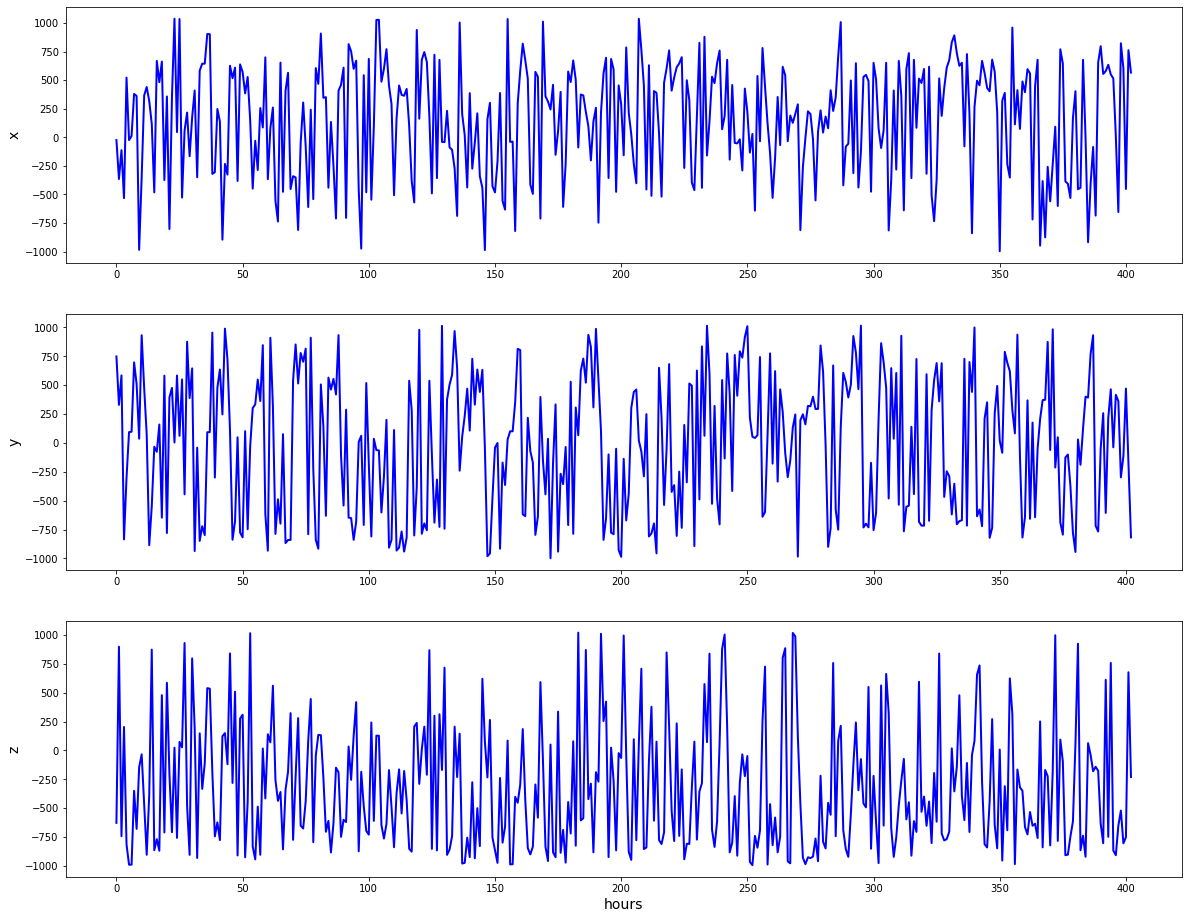
\includegraphics[scale=0.3]{img/task_1/data(hour).png}
  \caption{}
  \label{fig: }
\end{figure}

\textcolor{red}{TODO} caption figure

Let's take a look at the statistics of the dataset:

\begin{center}
\begin{tabular}{| c | c | c | c | c | c | c | c |} 
\hline
column & mean & std & min & 25\% & 50\% & 75\% & max \\ [0.5ex] 
\hline
\hline
x & 132.732967 & 491.697810 & -1239.0 & -291.0 & 214.0 & 539.0 & 1039.0 \\
\hline
y & -34.800146 & 594.977813 & -1019.0 & -646.0 & -14.0 & 466.0 & 1078.0 \\
\hline
z & -307.588768 & 538.335654 & -1001.0 & -794.0 & -416.0 & 83.0 & 1032.0 \\ [1ex]
\hline
\end{tabular}
\end{center}


\begin{figure}[H]
\centering
  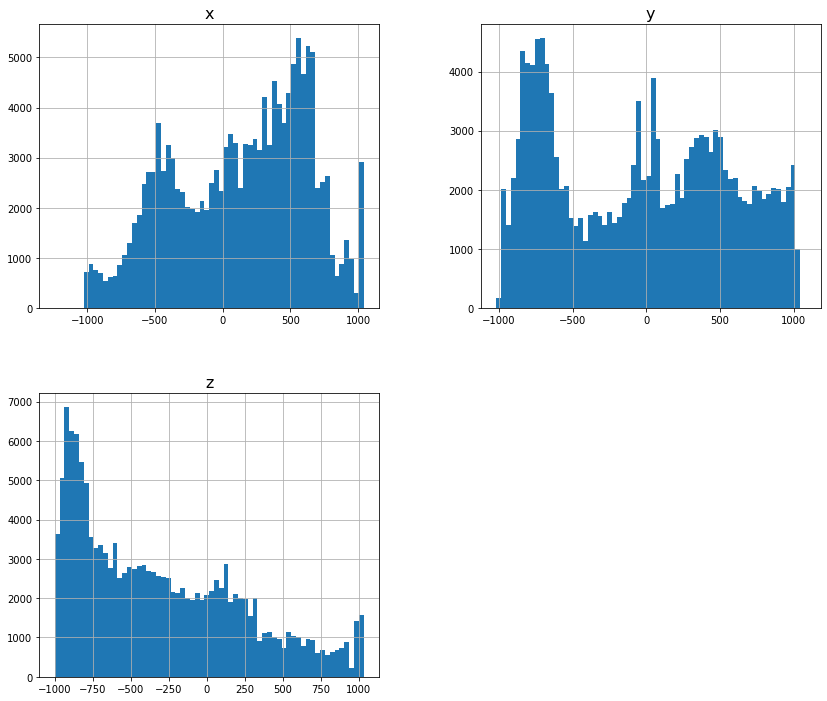
\includegraphics[scale=0.4]{img/task_1/histograms.png}
  \caption{}
  \label{fig: }
\end{figure}

\textcolor{red}{TODO} caption figure





\addcontentsline{toc}{section}{Data Preparation}
\section*{Data Preparation}\label{Data Preparation}

\addcontentsline{toc}{subsection}{Splitting}
\subsection*{Splitting}\label{Splitting}

~~We'll use a 80\% of the train data (train.csv) for training and remaining 20\% for validation. The test data (test.csv) was set aside for testing the model.

\begin{lstlisting}[language=Python]
import pandas as pd

train_data = pd.read_csv('train.csv', sep = ',')
test = pd.read_csv('test.csv', sep = ',')

n = len(train)

train = train_data[           : int(n*0.8)]
valid = train_data[int(n*0.8) :           ]
\end{lstlisting}

\addcontentsline{toc}{subsection}{Scaling}
\subsection*{Scaling}\label{Scaling}

~~We'll transform each feature individually such that it is in the given range on the training set, in our case between -1 and 1. This transformation is often used as an alternative to zero mean, unit variance scaling.

\begin{lstlisting}[language=Python]
from sklearn.preprocessing import MinMaxScaler

scaler = MinMaxScaler(feature_range=(-1,1))

train = scaler.fit_transform(train_df)
valid = scaler.transform(valid_df)
\end{lstlisting}

\addcontentsline{toc}{subsection}{Windowing}
\subsection*{Windowing}\label{Windowing}

~~Our model will make a set of predictions based on a window of consecutive samples from the data. The main features of the input windows are:

\begin{itemize}
  \item[1.] the window size (number of time steps) of the input and
  \item[2.] the window shift.
\end{itemize}

For example, to make a single prediction 1 minute into the future, given 5 minutes of history, we might define a window like this:

Suppose that x has these values: x = [0, 1, 2, 3, 4]. Assume that the size of the window is 2 and the shift is 1. We create the following sequences: data = [[0, 1], [1, 2], [2, 3]], , label = [[2], [3], [4]], the goal is to predict for the sequence [0, 1] the value 2, for [1, 2] the value [3] and fot the sequence [2, 3] the value [4].


\begin{lstlisting}[language=Python]
def split(data, win_size=30, win_shift=6, offset=1):

  rows = np.arange(win_size, len(data) - win_shift - 1, win_shift)

  samples = np.zeros((len(rows), win_size, data.shape[-1]))
  targets = np.zeros((len(rows),))

  for j, row in enumerate(rows):
    samples[j] = data[j * win_shift: row]
    targets[j] = data[row: row + offset]

  return samples, targets
\end{lstlisting}





\addcontentsline{toc}{section}{Data Modeling}
\section*{Data Modeling}\label{Data Modeling}

~~Time series prediction problems are a difficult type of predictive modeling problem. Unlike regression predictive modeling, time series also adds the complexity of a sequence dependence among the input variables. A powerful type of neural network designed to handle sequence dependence is called Recurrent Neural Network (RNN). 

When reading a sentence the human brain processes it word by word while keeping memories of what came before; this gives humans a fluid representation of the meaning conveyed by the sentence. Biological intelligence processes information incrementally while maintaining an internal model of what it’s processing, built from past information and constantly updated as new information comes in.

A RNN adopts the same principle, albeit in an extremely simplified version: it processes sequences by iterating through the sequence elements and maintaining a state containing information relative to what it has seen so far. In effect, an RNN is a type of neural network that has an internal loop. The state of the RNN is reset between processing two different, independent sequences, so you still consider one sequence a single data point: a single input to the network. What
changes is that this data point is no longer processed in a single step; rather, the network internally loops over network: a network with a loop sequence elements.

Susch RNNs have a major issue: although it should theoretically be able to retain at time t information about inputs seen many timesteps before, in practice, such long-term dependencies are impossible to learn. This is due to the vanishing gradient problem, an effect that is similar to what is observed with non-recurrent networks (feedforward networks) that are many layers deep: as you keep adding layers to a network, the network eventually becomes untrainable. Long Short-Term Memory (LSTM) networks tackle this problem. LSTM network adds a way to carry information across many timesteps thus preventing older signals from gradually vanishing during processing. We will use this type of netkwork for modeling our data.

An important constructor argument for all Keras RNN layers, such as tf.keras.layers.LSTM, is the return\_sequences argument. This setting can configure the layer in one of two ways:

\begin{itemize}
  \item[1.] If False, the default, the layer only returns the output of the final time step, giving the model time to warm up its internal state before making a single prediction:
\end{itemize}


\begin{figure}[H]
\centering
  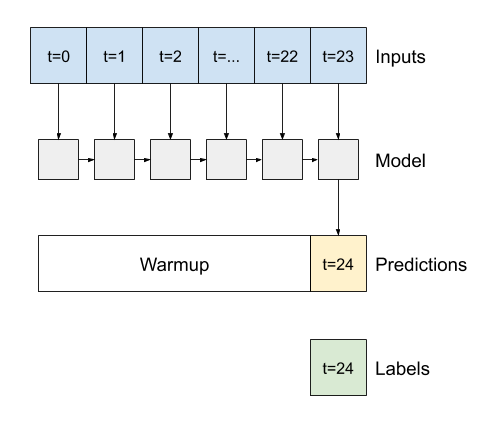
\includegraphics[scale=0.35]{img/task_1/fig1.png}
  \caption{}
  \label{fig: }
\end{figure}

\textcolor{red}{TODO} caption figure

\begin{itemize}
  \item[1.] If True, the layer returns an output for each input. This is useful for:
  \begin{itemize}
     \item[a)] Stacking RNN layers.
     \item[b)] Training a model on multiple time steps simultaneously.
   \end{itemize}
\end{itemize}

\begin{figure}[H]
\centering
  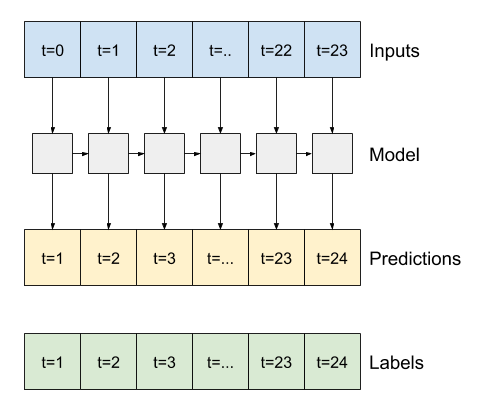
\includegraphics[scale=0.35]{img/task_1/fig2.png}
  \caption{}
  \label{fig: }
\end{figure}

\textcolor{red}{TODO} caption figure

Here is our model.

\begin{lstlisting}[language=Python]
lstm = tf.keras.models.Sequential([
	tf.keras.layers.LSTM(16, 
			     input_shape=(seq_len, num_feat), 
			     return_sequences=True),
	tf.keras.layers.LSTM(8),
	tf.keras.layers.Dense(1, activation='tanh')
])
\end{lstlisting}

\begin{lstlisting}[language=Python]
lstm.compile(loss = 'mae', optimizer='adam')

history = lstm.fit(x_train, y_train, epochs=100, 
			validation_data=(x_valid, y_valid), 
			verbose = 1, batch_size=32, shuffle=False)
\end{lstlisting}

\begin{center}
\begin{tabular}{| c | c | c | c |} 
\hline
 & x & y & z  \\ [0.5ex] 
\hline
\hline
MAE & 54.55 & 59.22 & 61.74 \\
\hline
\end{tabular}
\end{center}

\begin{center}
\begin{tabular}{| c | c |} 
\hline
Window (min) & MAE  \\ [0.5ex] 
\hline
\hline
 1 & 65.14 \\
 \hline
 2 & 55.27 \\
 \hline
 3 & 63.99 \\
 \hline
 4 & 55.63 \\
 \hline
 5 & 60.96 \\
 \hline
 6 & 55.34 \\
 \hline
 7 & 63.05 \\
 \hline
 8 & 58.61 \\
 \hline
 9 & 55.33 \\
 \hline
 10 & 54.85 \\
 \hline
 11 & 54.47 \\
 \hline
 12 & 55.03 \\
 \hline
 13 & 58.72 \\
 \hline
 14 & 54.69 \\
 \hline
 15 & 64.59 \\
\hline
\end{tabular}
\end{center}

\begin{center}
\begin{tabular}{| c | c |} 
\hline
Shift (min) & MAE  \\ [0.5ex] 
\hline
\hline
0.5 & 61.46\ \\
\hline
1 & 57.68\ \\
\hline 
1.5 & 57.92\ \\
\hline 
2 & 55.09 \\
\hline 
2.5 & 54.76\ \\
\hline 
3 & 54.62 \\
\hline 
3.5 & 58.28 \\
\hline 
4 & 57.29\ \\
\hline 
4.5 & 60.71 \\
\hline 
5 & 56.14 \\
\hline
5.5 & 59.64 \\
\hline 
6 & 55.21 \\
\hline
6.5 & 60.45 \\
\hline
7 & 58.58 \\
\hline 
7.5 & 53.86 \\
\hline
\end{tabular}
\end{center}


\addcontentsline{toc}{chapter}{Anomaly detection}
\chapter*{Anomaly detection}

\addcontentsline{toc}{section}{Data Understanding}
\section*{Data Understanding}\label{Data Understanding}

~~The training set is composed by control patient, i.e. volunteers without Parkinson’s Desease. 

The train dataset contains 7 different features: identification of patient, accelerometer readings in the three axes (x, y, z), heart rate, date and timestamp. Data were collected every 1 seconds for a total of 943522 records and 13 volunteers. Missing value on heart rate attribute are labeled with -1.

Here are the first few rows of the train dataset:

\begin{center}
\begin{tabular}{| c | c | c | c | c | c | c | c |} 
\hline
No. & patient & x & y & z & heartRate & timestamp & tsDate \\ [0.5ex] 
\hline
\hline
0 &	1502 &	23 &	569 &	878 &	-1 &	1568073600000 &	2019-09-10 00:00:00.003 \\
\hline
1 &	1502 &	23 &	571 &	878 &	-1 &	1568073601000 &	2019-09-10 00:00:01.014 \\
\hline
2 &	1502 &	23 &	570 &	878 &	-1 &	1568073602000 &	2019-09-10 00:00:02.025 \\
\hline
3 &	1502 &	23 &	570 &	878 &	-1 &	1568073603000 &	2019-09-10 00:00:03.035 \\
\hline
4 &	1502 &	23 &	570 &	878 &	-1 &	1568073604000 &	2019-09-10 00:00:04.046 \\
\hline
5 &	1502 &	23 &	570 &	879 &	-1 &	1568073605000 &	2019-09-10 00:00:05.057 \\
\hline
6 &	1502 &	23 &	569 &	879 &	-1 &	1568073606000 &	2019-09-10 00:00:06.066 \\
\hline
7 &	1502 &	22 &	570 &	879 &	-1 &	1568073607000 &	2019-09-10 00:00:07.078 \\
\hline
8 &	1502 &	23 &	570 &	879 &	-1 &	1568073608000 &	2019-09-10 00:00:08.088 \\
\hline
9 &	1502 &	24 &	570 &	878 &	-1 &	1568073609000 &	2019-09-10 00:00:09.099 \\ [1ex] 
\hline
\end{tabular}
\end{center}

Here is the time evolution of the three components of acceleration and heart rate over time for one volunteer:

\begin{figure}[H]
\centering
  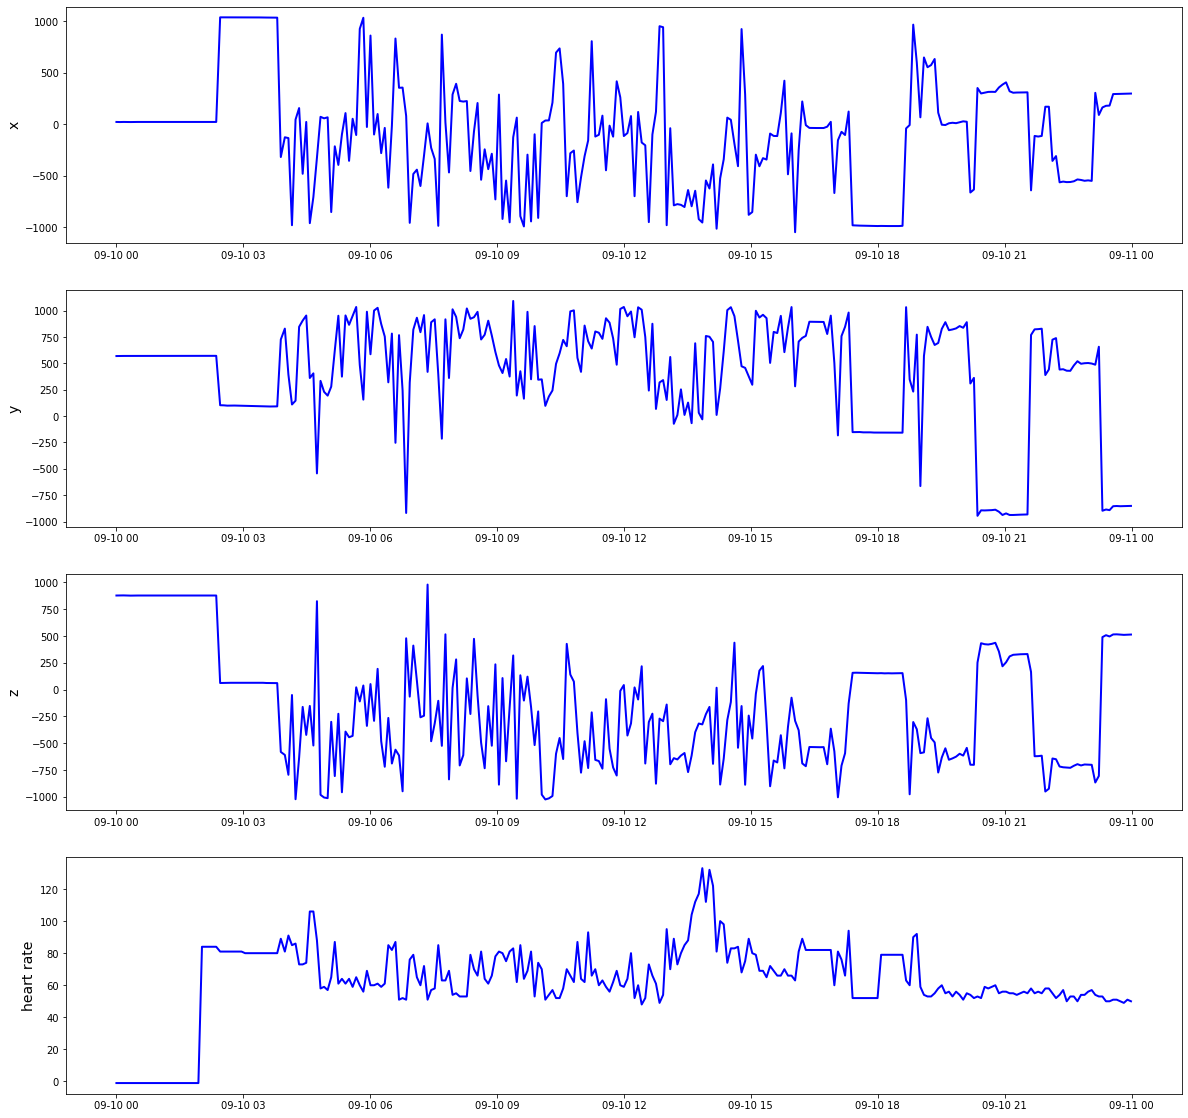
\includegraphics[scale=0.3]{img/task_2/data(5min).png}
  \caption{Time evolution of the three components of acceleration and heart rate over time for one volunteer}
  \label{fig: fig: time evolution acc and hr task 2}
\end{figure}

Let's take a look at the statistics of the dataset:

\begin{center}
\begin{tabular}{| c | c | c | c | c | c | c | c |} 
\hline
column & mean & std & min & 25\% & 50\% & 75\% & max \\ [0.5ex] 
\hline
\hline
x  &	-82.99378 & 577.0332 & -1649.000  & -532.0000 & -91.00000 & 311.0000 & 1796.000 \\
\hline
y  &	265.3513 & 539.7477 & -1082.000 & -59.00000 & 313.0000 & 7.390000 & 1644.000 \\
\hline
z  &	-203.9305 & 534.9554 & -1256.0003  & -665.0000 & -223.0000  & 125.0000 & 1127.000 \\
\hline
heartRate & 70.20357 & 20.97376 & -1.000000 & 61.000001 & 70.00000 & 82.00000 & 182.0000 \\ [1ex]
\hline
\end{tabular}
\end{center}

\begin{figure}[H]
\centering
  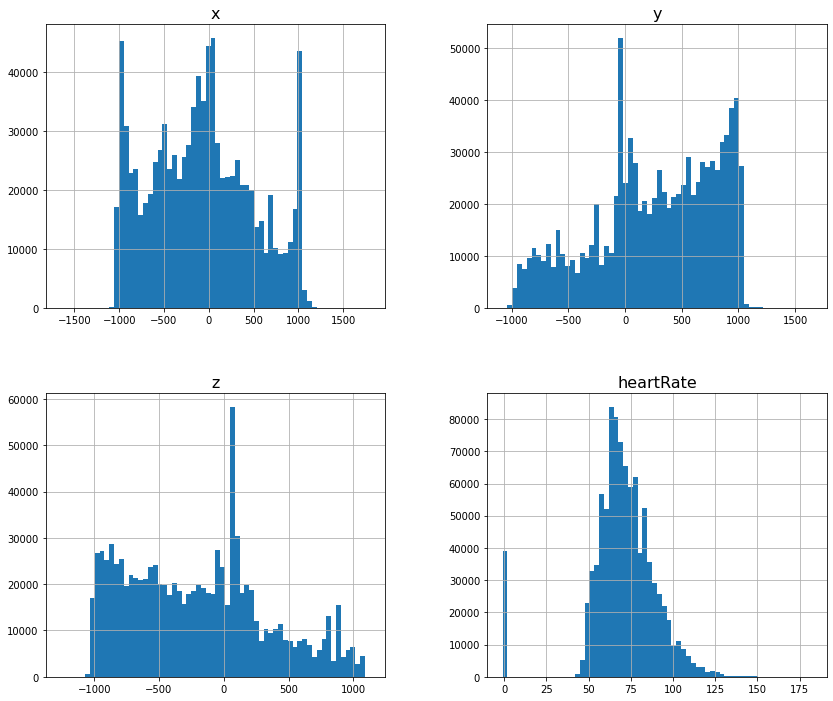
\includegraphics[scale=0.4]{img/task_2/histograms.png}
  \caption{Distribution of the data.}
  \label{fig: histograms task 2 }
\end{figure}





\addcontentsline{toc}{section}{Data Preparation}
\section*{Data Preparation}\label{Data Preparation}

~~First, we replace missing values on heart rate attribute (labeled with -1) with median.

\begin{lstlisting}[language=Python]
import pandas as pd

trn_df = pd.read_csv('ad_train.csv', sep = ',')
tst_df = pd.read_csv('ad_test.csv', sep = ',')

bad_hr = trn_df['heartRate'] == -1
trn_df['heartRate'][bad_hr] = np.median(trn_df['heartRate'])
\end{lstlisting}

Select only relevant attributes meaning the three components of the acceleration and heart rate and sub-sample the data from 1 second interval to 10 second interval.

\addcontentsline{toc}{subsection}{Splitting}
\subsection*{Splitting}\label{Splitting}

~~As before we'll use a 80\% of the train data (ad\_train.csv) for training and the remaining 20\% for validation. The test data (ad\_test.csv) was set aside for testing the model.

\begin{lstlisting}[language=Python]
n = len(train_df)

train_data = train_df[           : int(n*0.8)].to_numpy()
valid_data = train_df[int(n*0.8) :           ].to_numpy()
test_data  = tst_df[['x', 'y', 'z', 'heartRate']].to_numpy()
\end{lstlisting}





\addcontentsline{toc}{subsection}{Scaling}
\subsection*{Scaling}\label{Scaling}

~~We'll transform each feature individually such that it is in the given range on the training set, in our case between 0 and 1. 

\begin{lstlisting}[language=Python]
from sklearn.preprocessing import MinMaxScaler

scaler = MinMaxScaler()

train = scaler.fit_transform(train_data.reshape(-1, 1))
valid = scaler.transform(valid_data.reshape(-1, 1))
test = scaler.transform(test_data.reshape(-1, 1))
\end{lstlisting}





\addcontentsline{toc}{section}{Data Modeling}
\section*{Data Modeling}\label{Data Modeling}

In anomaly detection, the goal is to find objects that do not conform to normal patterns or behavior. Often, anomalous objects are known as \textbf{outliers}, since, on a scatter plot of the data, they lie far away from other data points. Anomaly detection is also known as \textbf{deviation detection}, because anomalous objects have attribute values that deviate significantly from the expected or typical attribute values, or as \textbf{exception mining}, because anomalies are exceptional in some sense. There are a variety of anomaly detection approaches from several areas, including statistics, machine learning, and data mining. All try to capture the idea that an anomalous data object is unusual or in some way inconsistent with other objects.

Although unusual objects or events are, by definition, relatively rare, their detection and analysis provides critical insights that are useful in a number of
applications for instance in Medicine and Public Health. For a particular patient, unusual symptoms or test results may indicate potential health problems. However, whether a particular test result is anomalous may depend on many other characteristics of the patient, such as age, sex, and genetic makeup. Furthermore, the categorization of a result as anomalous or not incurs a cost—unneeded additional tests if a patient is healthy and potential harm to the patient if a condition is left undiagnosed and untreated. The detection of emerging disease outbreaks which result in unusual and alarming test results in a series of patients, is also important for monitoring the spread of diseases and taking preventive actions.

The nature of the input data plays a key role in deciding the choice of a suitable anomaly detection technique.

If the data contains a single attribute, the question of whether an object is anomalous depends on whether the object’s value for that attribute is anomalous. However, if the data objects are represented using many attributes, a data object may have anomalous values for some attributes but ordinary values for other attributes. Furthermore, an object may be anomalous even if none of its attribute values are individually anomalous. Identifying an anomaly in a multivariate
setting is thus challenging, particularly when the dimensionality of the data is high.

Since anomalies are infrequent, most input data sets have a predominance of normal instances. The input data set is thus often used as an imperfect representation of the normal class in most anomaly detection techniques. However, the performance of such methods needs to be robust to the presence of outliers in the input data.

Anomalies, unlike normal objects, are often unrelated to each other and hence distributed sparsely in the space of attributes. Indeed, the successful operation of most anomaly detection methods depends on anomalies not being tightly clustered.

\addcontentsline{toc}{subsection}{Reconstruction-based Approaches}
\subsection*{Reconstruction-based Approaches}\label{Reconstruction-based Approaches}

Reconstruction-based techniques rely on the assumption that the normal class resides in a space of lower dimensionality than the original space of attributes.
In other words, there are patterns in the distribution of the normal class that can be captured using lower-dimensional representations, e.g., by using dimensionality reduction techniques.

To illustrate this, consider a data set of normal instances, where every instance is represented using p continuous attributes, $x_1$, ... , $x_p$ . If there is
a hidden structure in the normal class, we can expect to approximate this data using fewer than $p$ derived features.

One common approach for deriving useful features from a data set is to use autoencoders. An autoencoder (also referred to as an autoassociator or a mirroring net-
work) is a multi-layer neural network, where the number of input and output neurons is equal to the number of original attributes. The general architecture of an autoencoder involves two basic steps: encoding and decoding. During encoding, a data instance $\textbf{x}$ is transformed to a low-dimensional representation $\textbf{y}$, using a number of nonlinear transformations in the encoding layers. The number of neurons reduces at every encoding layer, so as to learn low-dimensional representations from the original data. The learned representation $\textbf{y}$ is then mapped back to the original space of attributes using the decoding layers, resulting in a reconstruction of $\textbf{x}$ ($\hat {\textbf{x}}$). The distance between $\textbf{x}$ and $\hat {\textbf{x}}$ (the reconstruction error) is then used as a measure of an anomaly score.

The autoencoder scheme provides a powerful approach for learning complex and nonlinear representations of the normal class. We will use this approach to try to detect anomalies in our data.

Here is our model.

\begin{lstlisting}[language=Python]
encoder_inputs = 
	tf.keras.layers.Input(shape=(sequence_length, number_of_features))

encoder_l1 = tf.keras.layers.LSTM(16, return_state=True, activation='tanh')
encoder_outputs1 = encoder_l1(encoder_inputs)
encoder_states1 = encoder_outputs1[1:]

decoder_inputs = 
	tf.keras.layers.RepeatVector(sequence_length)(encoder_outputs1[0])

decoder_l1 = 
	tf.keras.layers.LSTM(16, return_sequences=True, activation='tanh')
	(decoder_inputs, initial_state = encoder_states1)

decoder_outputs1 = 
	tf.keras.layers.TimeDistributed(tf.keras.layers.Dense(number_of_features))
	(decoder_l1)

autoencoder = tf.keras.models.Model(encoder_inputs,decoder_outputs1)

autoencoder.summary()
\end{lstlisting}

\begin{lstlisting}[language=Python]
reduce_lr = tf.keras.callbacks.LearningRateScheduler(lambda x: 1e-3 * 0.90 ** x)

autoencoder.compile(loss = 'mae', optimizer='adam')
history = autoencoder.fit(train, train, epochs=60, 
		validation_data=(valid, valid), verbose=1, 
		batch_size=32, shuffle=False, callbacks=[reduce_lr])
\end{lstlisting}





\addcontentsline{toc}{subsection}{Detect Anomaly}
\subsection*{Detect Anomaly}\label{Detect Anomaly}

We will plot the train data, the reconstruction after it's encoded and decoded by the autoencoder, and the reconstruction error of the three components of acceleration and heart rate over time for one volunteer.

\begin{figure}[H]
\centering
  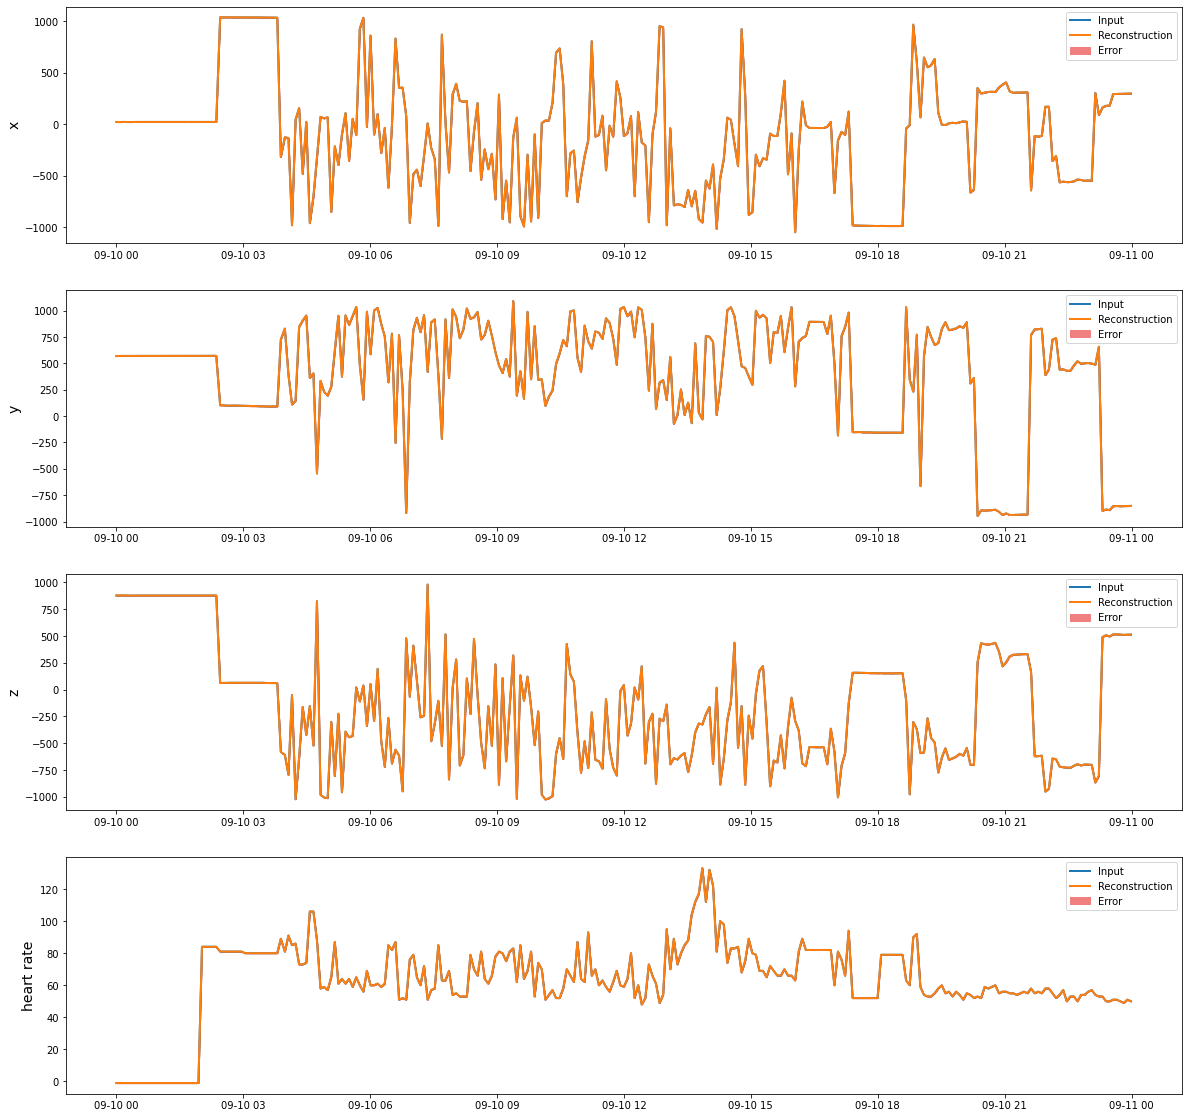
\includegraphics[scale=0.35]{img/task_2/reconstructions_train.png}
  \caption{Train data, the reconstruction and the reconstruction error of the three components of acceleration and heart rate over time for one volunteer.}
  \label{fig: rec train}
\end{figure}

We'll detect anomalies by calculating whether the reconstruction loss is greater than a fixed threshold.

We choose a threshold value then classify future examples as anomalous if the reconstruction error is higher than the threshold.

We will use three different thresholds values:

\begin{itemize}
  \item[1.] calculate the mean and standard deviation of the reconstruction error of the training set, then classify future examples as anomalous if the reconstruction error is higher than one standard deviation from the training set,
  \item[2.] calculte the third quartile, then classify future examples as anomalous if the reconstruction error is higher than  this value, 
  \item[3.] classify future examples as anomalous if the reconstruction error is higher than  0.003.
\end{itemize}

Let's take a look to the distribution of the reconstruction error on the train data.

\begin{figure}[H]
\centering
  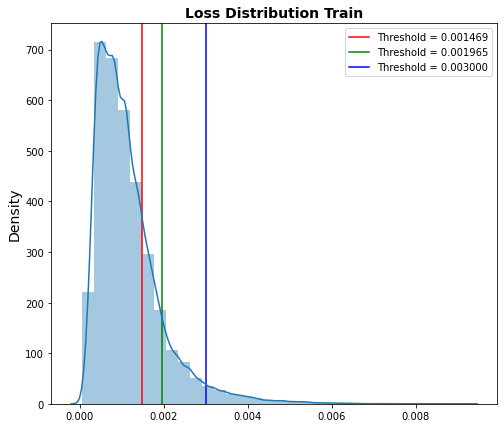
\includegraphics[scale=0.4]{img/task_2/train_loss.png}
  \caption{Distribution of reconstruction error on the train data and the three thresholds.}
  \label{fig: train loss}
\end{figure}

Then we applied our model to the test data and plot the reconstruction error on the test data alongside the reconstruction error on the train data and the thresholds.

\begin{figure}[H]
\centering
  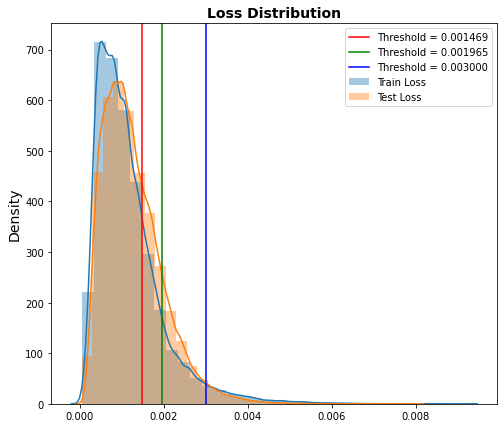
\includegraphics[scale=0.4]{img/task_2/train_test_loss.png}
  \caption{Distribution of reconstruction error on the test data and the three thresholds.}
  \label{fig: test loss}
\end{figure}

We will plot the test data, the reconstruction after it’s encoded and decoded by the autoencoder, and the reconstruction error of the three components of acceleration and heart rate over time for one patient.

\begin{figure}[H]
\centering
  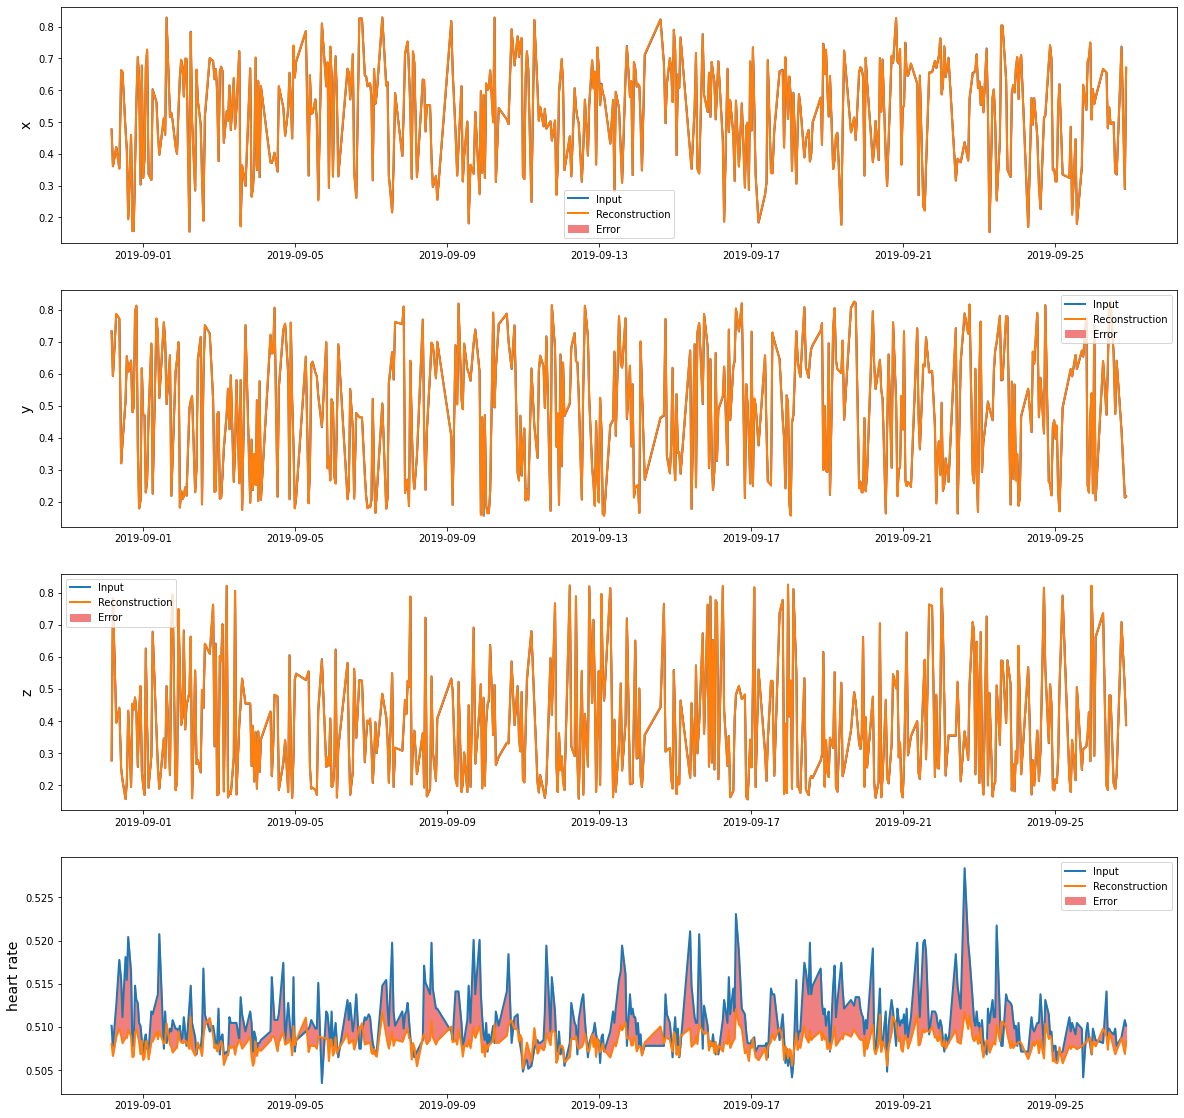
\includegraphics[scale=0.35]{img/task_2/reconstructions_test.png}
  \caption{Test data, the reconstruction and the reconstruction error of the three components of acceleration and heart rate over time for one patient(1004).}
  \label{fig: rec test}
\end{figure}

Finally for each row in the test set we will attach a label: true means that the row present normal values (reconstruction loss below the threshold) and false means that the row present anomaly values (reconstruction loss above the threshold). Here are a few rows.

\begin{center}
\begin{tabular}{| c | c | c | c | c | c | c |} 
\hline
No. & patient & tsDate & threshold=0.0014 & threshold=0.0019 & threshold=0.0030 \\ [0.5ex] 
\hline
\hline
0 &	1004 & 2019-08-31 04:00:00.004 & True & True & True \\
\hline
1 &	1004 & 2019-08-31 04:00:10.022 & True & True & True \\
\hline
2 &	1004 & 2019-08-31 04:00:20.041 & True & True & True \\
\hline
3 &	1004 & 2019-08-31 04:00:30.059 & True & True & True \\
\hline
4 &	1004 & 2019-08-31 04:00:40.060 & True & True & True \\
\hline
5 &	1004 & 2019-08-31 04:00:50.079 & True & True & True \\
\hline
6 &	1004 & 2019-08-31 04:01:00.099 & True & True & True \\
\hline
7 &	1004 & 2019-08-31 04:01:10.118 & True & True & True \\
\hline
8 &	1004 & 2019-08-31 04:01:20.136 & False & True & True \\
\hline
9 &	1004& 2019-08-31 04:01:30.145 & False & True & True \\ [1ex] 
\hline
\end{tabular}
\end{center}

\addcontentsline{toc}{chapter}{Conclusions}
\chapter*{Conclusions}

Our fist task was next value prediction, for that purpose we use an special type of recurrent neural network name Long Short Term Memory. We were able to predit the next value with a mean square error of 54.55, 59.22, 61.74 for x, y and z respectively using a window size of 5 minutes and a window shift of 1 minute. 

We repeat the calculation maintaining the window shift constant and varying the window size from 1 minute to 15 minutes one minute step, then maintaining the window size constant and varying the window shift half a minute step. Mean Absolute Error does not show any significant improvement.

Our second task was to detect anomalies, for that purpose we use an autoencoder to learn a representation of the train data assuming it was normal, then we decide whether a data point was normal or anomalous based on how well our model performs over the test data. We produce a file (.csv) in which for each patients we insert the dates in which an anomalous behaviour occurs.


\end{document}
